\chapter{ESTUDO DE CASO}
Este capítulo apresenta um estudo de caso da implementação de uma ferramenta de documentação executável no projeto da Biblioteca Digital.

O estudo de caso foi idealizado devido a necessidade de existir uma documentação que agregue mais valor ao cliente. Documentação executável pode validar requisitos e guiar o usuário no emprego do sistema.

\section{Projeto da Biblioteca Digital} 	 	

A Biblioteca Digital (BD) é um projeto de pesquisa e desenvolvimento que inciou-se em março de 2007, através de uma solicitação da SETEC/MEC ao Núcleo de Pesquisa de Sistemas de Informação (NSI) do Instituto Federal Fluminense. O NSI foi criado em abril de 2002 e desde essa época vem estimulando o uso tecnologias livres para pesquisa e desenvolvimento de software.

O projeto da BD visa disponibilizar um acervo de documentos produzidos pela rede de Instituições de Educação Profissional Científica e Tecnológica (EPCT) – como artigos, monografias, dissertações, teses e periódicos – promovendo a disseminação de conhecimento através destes conteúdos.

Como em todo projeto de desenvolvimento de software, a documentação do sistema é um problema constante. Sincronizar documentos escritos em papel com o código do sistema, é uma tarefa difícil e sujeita a falhas. 

\section{Proposta da ferramenta}

Devido a este problema, foi levantada a necessidade de desenvolver uma ferramenta de documentação executável que permita ao usuário validar requisitos do sistema e guiá-lo na utilização do mesmo. Portanto esta ferramenta tem como objetivos suportar sua documentação e treinar o usuário no emprego do sistema.

Assim, pode-se destacar como vantagens da implantação a otimização do uso do sistema, pois através dos passos estabelecidos o usuário poderá avaliar a simplicidade da execução das ações ou estabelecer outros comportamentos melhorados.

Outra vantagem esperada é a validação dos cenários, onde todos os passos executados foram pré-definidos pela especificação do cliente. Desta maneira pode-se validar interativamente todos os cenários descritos.

A partir da utilização da documentação interativa, os usuários poderão ser facilmente treinados nas funcionalidades da Biblioteca Digital, sem a necessidade de uma tutoria dedicada.

\section{Desenvolvimento}

Neste tópico serão demonstrados os passos executados para realização deste trabalho, possibilitando ao leitor avaliar ou reproduzir os efeitos aqui descritos.

\subsection{Ambiente de desenvolvimento}

O projeto da BD é desenvolvido na linguagem \textit{Ruby} utilizando o \textit{framework} \textit{web Ruby on Rails} \cite{RAILS}. Uma das vantagens de utilizar este \textit{framework} é a existência de um conjunto de bibliotecas que facilitam o desenvolvimento guiado a testes \cite{BECK}.

Durante o processo de desenvolvimento da ferramenta foi utilizada a biblioteca de testes automatizados RSpec \cite{CHELIMSKY}, a qual fornece ao desenvolvedor uma \textit{domain specific language} (DSL), que facilita especificação dos comportamentos esperados do objeto (Código \ref{lst:codigo31}).

{\singlespace
\begin{lstlisting}[caption=Exemplo da DSL do Rspec,label={lst:codigo31}]
describe Person do
  subject {
    Person.new(:name => "John Doe", :role => "moderator")
    }

  its(:name) { should == "John Doe" }

  it "is a admin" do
    subject.role = "admin"
    subject.should be_admin
  end

  it "is not a admin" do
    subject.role = nil
    subject.should_not be_admin
  end

  it "instantiates without hash" do
    expect { Person.new }.to_not raise_error(ArgumentError)
  end
end
\end{lstlisting}
}

O resultado de execução do código acima pode ser visto na Figura \ref{figura_31}, a qual descreve os testes que passaram.

\begin{figure}[ht]
    \centering
    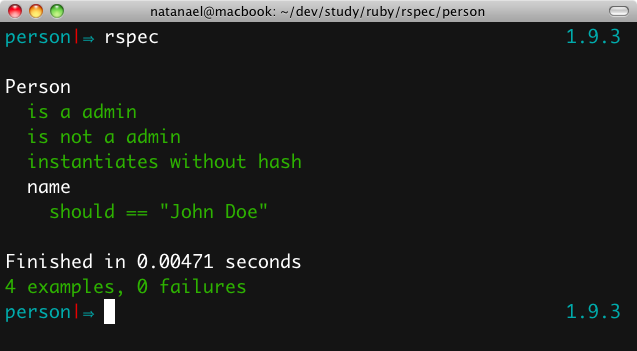
\includegraphics[width=0.9 \textwidth]{figuras/figura_31}
    \caption{Saída após rodar os testes com RSpec}
    \label{figura_31}
\end{figure}

Além da utilização desta biblioteca de testes, foi utilizado o conceito de "passos de bebê", ou seja, pequenas partes são desenvolvidas a cada momento, seja levantamento de requisitos, implementação de funcionalidade, refatoração ou até especificações. Um exemplo disto é focar no desenvolvimento de uma pequena parte de uma funcionalidade, diminuindo o risco do desenvolvimento e asegurando o atingimento de objetivos alcançaveis \cite{RODRIGO}.

\subsection{Testes desenvolvidos}

Todo processo de desenvolvimento da ferramenta utilizou TDD, onde foram criadas verificações unitárias dos \textit{models}, \textit{views} e \textit{controllers}.

Os testes de \textit{model} têm a responsabilidade de especificar e verificar a lógica de negócio da aplicação, avaliando o comportamento dos objetos. O Código \ref{lst:codigo33} mostra o teste responsável pelo \textit{model} \textit{Scenario}.

{\singlespace
\begin{lstlisting}[caption=Teste unitário de \textit{model},label={lst:codigo33}]
describe Scenario do
  it { should_not have_valid(:yaml).when('', nil) }
  its(:yaml) { should be_accessible }

  context "when a yaml file" do
    context "is not given" do
      its(:name) { should eq('') }
      its(:to_param) { should eq("") }
      its(:contexts) { should eq([]) }
      its(:to_hash) { should be_empty }
      its(:to_hash) { should be_a(Hashr) }
    end

    context "is given" do
      subject { Scenario.new yaml: File.read("./spec/resources/scenario.yml") }

      it "#to_hash should return @yaml Hashr" do
        subject.yaml = "hero: _why"
        subject.to_hash.should eq({:hero => '_why'})
        subject.to_hash.should be_a(Hashr)
      end

      it "#url should return the first context url" do
        subject.stub(id: 1)
        subject.url.should eq("/?tourId=1-criar-usuario")
      end
    end
  end
end
\end{lstlisting}
}

A cobertura de testes atumatizados das \textit{views} foram desenvolvidas para verificar se o conteúdo é corretamente apresentado ao usuário na página (Código \ref{lst:codigo34}).

{\singlespace
\begin{lstlisting}[caption=Teste unitário de \textit{view},label={lst:codigo34}]
describe "scenarios/_context.html.erb" do
  before do
    render "scenarios/context",
      context: Hashr.new(url: '/', steps: [mock.as_null_object, mock.as_null_object])
  end

  it "render context div" do
    rendered.should have_selector("div[title='/']")
  end

  it "should render _step for each step" do
    rendered.should render_template(partial: 'scenarios/_step', count: 2)
  end
end
\end{lstlisting}
}

No caso dos \textit{controllers}, foram avaliados os comportamentos das classes controladoras da aplicação, as quais somente repassam requisições entre \textit{model} e \textit{view} (Código \ref{lst:codigo35}).

{\singlespace
\begin{lstlisting}[caption=Teste unitário de \textit{controller},label={lst:codigo35}]
describe ApplicationController do
  describe "before_filter" do
    controller do
      def index
        render nothing: true
      end
    end

    context "when params[:tourId] is valid" do
      let (:scenario) { stub_model(Scenario, id: 1, name: 'Add user') }
      before do
        Scenario.stub(:find_by_id).with("1-add-user").and_return(scenario)
        get :index, tourId: "1-add-user"
      end

      it "load @current_scenario if params[:tourId] is valid" do
        assigns[:current_scenario].should eq(scenario)
      end

      it "create cookie with Scenario#to_param" do
        cookies[:ajcookie_tourId].should eq(scenario.to_param)
      end
    end
  end
end
\end{lstlisting}
}

\subsection{Arquitetura da ferramenta}

O projeto inicial levou a construção de uma arquitetura onde os elementos constituintes da ferramenta se relacionavam conforme o modelo apresentado na Figura \ref{figura_32}.

\begin{figure}[ht]
    \centering
    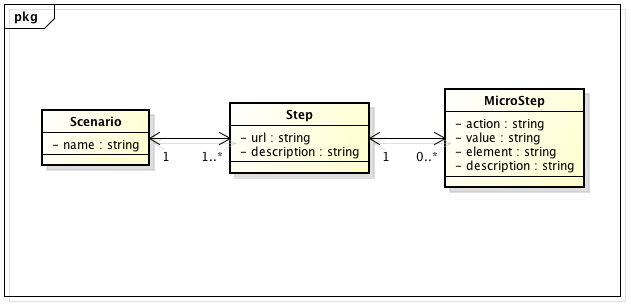
\includegraphics[width=0.9 \textwidth]{figuras/figura_32}
    \caption{Diagrama de classes da arquitetura inicial}
    \label{figura_32}
\end{figure}

Entretanto, após implementada esta arquitetura pode-se verificar a dificuldade na utilização da ferramenta. Foi então realizado um refatoramento que levou a descoberta de uma biblioteca da linguagem \textit{Ruby} (\textit{Hashr}) que facilitou uma nova arquitetura.

A biblioteca \textit{Hashr} cria uma nova classe derivada da classe \textit{Hash}, que simplifica o uso de \textit{hashes} aninhados e acesso aos seus valores \cite{HASHR}. O Código \ref{lst:codigo36} exemplifica o uso desta estrutura.

{\singlespace
\begin{lstlisting}[caption=Exemplo de uso da estrutura \textit{Hashr},label={lst:codigo36}]
monografia = Hashr.new titulo: 'Documentacao Executavel',
                       autores: {autor_1: 'Tiago', autor_2: 'Natanael'}

monografia.titulo  # => 'Documentacao Executavel'
monografia.autor_1 # => 'Tiago'
monografia.autor_2 # => 'Natanael'

\end{lstlisting}
}

Porém o exemplo acima não é a melhor representação da estrutura desejada. Os autores devem pertencer a uma lista, entretanto o \textit{Hashr} não converte os itens da lista conforme esperado. Para resolver este problema, foi desenvolvido um método recursivo que converte os valores em lista produzindo assim os efeitos esperados (Código \ref{lst:codigo37}).

{\singlespace
\begin{lstlisting}[caption=Método de conversão para \textit{Hashr},label={lst:codigo37}]
monografia = Hashr.new titulo: 'Documentacao Executavel',
                       autores: [{nome: 'Tiago'}, {nome: 'Natanael'}]

monografia.autores.first.nome # => NoMethodError

def convert_to_hashr(hash)
 hash = Hashr.new(hash)
 hash.values.find_all { |value| value.is_a?(Array) }.each do |value|
   value.each_index do |i|
     value[i] = convert_to_hashr(value[i]) if value[i].is_a? Hash
   end
 end
 hash
end

monografia = convert_to_hashr(monografia)
monografia.autores.first.nome  # => 'Tiago'
\end{lstlisting}
}

Com essa abordagem, foi possível criar uma estrutura simples de dicionários e listas para representar as classes \textit{Step} e \textit{MicroStep}, visto que essas classes eram pobres de lógica e serviam apenas para a estruturação e persistência de dados. Com essa estrutura foi possível fazer a simplificação da entrada de dados para o cadastro e gerenciamento dos cenários, usando o formato de serialização de dados \textit{YAML}.

A vantagem de utilizar este formato é que ele pode ser facilmente entendível por humanos e ao mesmo tempo é flexível e facilmente manipulável. Ele aceita representação para as estruturas de listas, dicionários e valores simples, como texto e inteiros \cite{YAML}. Usando esse formato de entrada, o cadastro de um novo cenário pode ser feita como exemplificado no Código \ref{lst:codigo38}.

{\singlespace
\begin{lstlisting}[caption=Exemplo de cenário escrito em \textit{YAML},label={lst:codigo38}]
scenario: Login de Usuario

contexts:
  - url: /
    steps:
      - description:
          Os links referentes ao acesso do usuario
          ficam no menu do canto superior direito
        element: actions
        padding: 3
        position: rmb

      - description: Clique na opcao 'Acesso'
        element: sign_in
        padding: 3
        position: rmb
        action: click

  - url: /usuarios/login
    steps:
      - description: Preencha o campo 'E-mail'
        element: usuario_email
        padding: 3
        position: tcc
        action: type
        value: exemplo@exemplo.com
      - description: Preencha o campo 'Senha'
        element: usuario_senha
        padding: 3
        position: tcc
        action: type
        value: exemplo123
      - description: Clique no botao 'Entrar'
        element: login
        padding: 3
        position: tcc
        action: click
\end{lstlisting}
}

